\documentclass[final]{beamer}
%\usepackage{mathabx}
\usepackage{arev}

\usepackage{amsmath,amsthm,amssymb,latexsym,bbding}
\everymath{\displaystyle}
\usepackage{mathtools}
% \boldmath

\usepackage[utf8]{inputenc}
\usepackage{csquotes}
\usepackage[english]{babel}
\usepackage[T1]{fontenc}
\usepackage[orientation=portrait,size=custom, height=97,width=97,scale=0.93,debug]{beamerposter}
\mode<presentation>
  {
  \usetheme{IPFposter}
  }


%%%%%%%%%%%%%%%%%%%%%%%%%%%%%%%%%%%%%%%%%%%%%%%%%%%%%%%%%%%%%%%%%%%%%%%%%%%%%%
%% definitions for this poster only



%%%%%%%%%%%%%%%%%%%%%%%%%%%%%%%%%%%%%%%%%%%%%%%%%%%%%%%%%%%%%%%%%%%%%%%%%%%%%%
%% biblatex

\usepackage[backend=biber,citestyle=numeric-comp,bibstyle=BIBStyle,%
            sorting=none,doi=false,hyperref=false]{biblatex}
\bibliography{thebib}
\setbeamertemplate{bibliography item}[text]  % set bibliography item, to show 
                                             % the text of the item (as it 
                                             % comes from biblatex);
                                             % otherwise we get these little 
                                             % images



%%%%%%%%%%%%%%%%%%%%%%%%%%%%%%%%%%%%%%%%%%%%%%%%%%%%%%%%%%%%%%%%%%%%%%%%%%%%%%
%% length and layout fig

\newlength{\columnheight}
\setlength{\columnheight}{97cm}

\setlength\textwidth{\paperwidth}

\newlength{\marginw}
\setlength{\marginw}{2cm}

\newlength{\tw}
\setlength{\tw}{\textwidth}
\addtolength{\tw}{-2\marginw}


\newlength{\colsep}
\setlength{\colsep}{2cm}

\newlength{\colw}
\setlength{\colw}{0.5\tw}
\addtolength{\colw}{-\colsep}


\setlength{\parindent}{0pt}

\setbeamersize{text margin left=0pt,%
text margin right=0pt,%
%sidebar width left=0pt,%
%sidebar width right=0pt,%
%description width=0pt,%
%description width of=0pt,%
%mini frame size=0pt,%
%mini frame offset=0pt%
}

\newenvironment{myTwoColPoster}{%
  \begin{minipage}[t]{\textwidth}%
    \hspace*{\marginw}%
    \hspace*{9.5bp}%  %% dirty trick!!!!
    %\hfill%
    \begin{minipage}[t]{\tw}}%
  {\end{minipage}%
   \hspace*{\marginw}%
   %\hfill%
   \end{minipage}}

\newenvironment{myCol}%
    {\begin{minipage}[t][\columnheight][t]{\colw}}%
    {\end{minipage}}

\newenvironment{textblock}[1]%
    {\begin{block}{\rule[-0.6ex]{0pt}{2.4ex}\raisebox{-0.25ex}[1.6ex]{#1}}%
     \vspace*{5mm}}%
    {\vspace*{5mm}\end{block}}


%%%------------------------------------------------------------------------%%%
%% the document
%%--------------------------------------------------------------------------%%

%% logos
\logoleft{
\includegraphics[keepaspectratio=true,width=9cm]{fig/logos/dd1_1.pdf}}
\logoright{
\includegraphics[keepaspectratio=true,width=9cm]{fig/logos/dd1_2.pdf}}

%% title
  \title[Fraktal Poster4]{{\huge Fraktale Dimensionen}}
  \author[]{\Large Martin Wengenmayr\inst{1,2} \and Ron Dockhorn\inst{1}
    \and Dirk Romeis\inst{1} \and Jens-Uwe Sommer\inst{1,2}} \institute[IPFdd UBS]{ \inst{1}Leibniz-Institut f\"ur
    Polymerforschung Dresden e. V., Hohe Stra\ss e
    6, 01069 Dresden\\
    \inst{2}TU Dresden, Intitut für Theoretische Physik, 01062 Dresden\\
    ~\vspace{1ex} } \date{}

%% set text in footline
\footlinetext{\texttt{http://www.ipfdd.de}\hfill\texttt{wengenmayr@ipfdd.de, dockhorn@ipfdd.de, romeis@ipfdd.de}}


%% replace altert{xx} command :
 %  "(\ \textcolor{IPForange}{.*?} )"  -->  " $1 "

%%--------------------------------------------------------------------------%%
%% content
\begin{document}
\begin{frame}[t]{}
\begin{myTwoColPoster}
% ---------------------------------------------------------%
% first column
\begin{myCol}
  \begin{textblock}{Was ist die Dimension?}
    \renewcommand{\baselinestretch}{1.2}
    \Large
    \textbf{  \textcolor{IPForange}{Intuitiv} } klar welche Dimension ein \textit{einfaches} geometrisches Objekt besitzt\\
    \begin{center}
      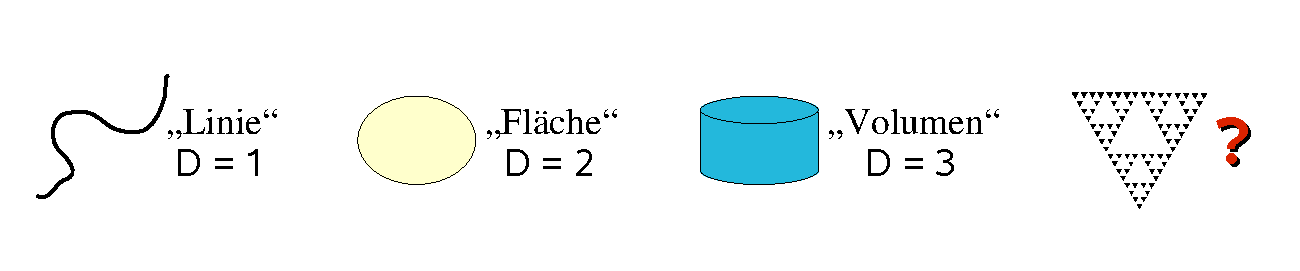
\includegraphics[width=0.96\textwidth]{fig/bsp}
    \end{center}
    Welche \textit{Länge} hat eine Kugel? Welches \textit{Volumen} hat ein Rechteck? \\
    \textcolor{IPForange}{$\boldsymbol{\Rightarrow}$} \textbf{Größenmaß} passt nicht zu \textbf{Objekt} \\
    Größe eines Objektes nur sinnvoll definiert im Bezug auf seine Dimension\\[1cm] % $\boldsymbol{ D_\text{f}}$\\[2cm]
    \textbf{  \textcolor{IPForange}{Mathematisch} } muss die Dimension $D$ eindeutig formuliert werden
    \begin{minipage}[c]{0.7\textwidth}
      \begin{itemize} \setlength\itemsep{1.1em} \Large
        \item Ausgangsfrage: Wie groß ist Dimension des Raumes, den Objekt ausf\"ullt ? 
        \item typische Ausdehnung $r$ : Abmessung in einer Richtung\\[2cm]
        \begin{itemize}\setlength\itemsep{1.3em} \Large 
          \item \textit{ Gr\"o\ss e} einer \textbf{Linie}   $l \sim r$
          \item \textit{ Gr\"o\ss e} eines \textbf{Kreises} $A \sim r^2$
          \item \textit{ Gr\"o\ss e} einer \textbf{Kugel}   $V \sim r^3$\\[1.2em]
          \textcolor{IPForange}{$\boldsymbol{\Rightarrow}$} \textbf{allgemein: $G_\text{d} \sim r^d$}
        \end{itemize}
      \end{itemize}
    \end{minipage}
    \hfill
    \begin{minipage}[c]{0.29\textwidth}
      \begin{center}
        \includegraphics[width=0.99\textwidth]{fig/groessen}
      \end{center}
    \end{minipage}
    
    \begin{center}
      \textbf{  \textcolor{IPForange}{Idee:} }Wie viele Kopien $N$ braucht man, f\"ur doppelte Gr\"o\ss e $G\,$?\\
      $\Rightarrow$ $G\to2\,G$\hspace*{1.5cm}durch\hspace*{1.5cm}$N=2^D$ Kopien
    \end{center}

    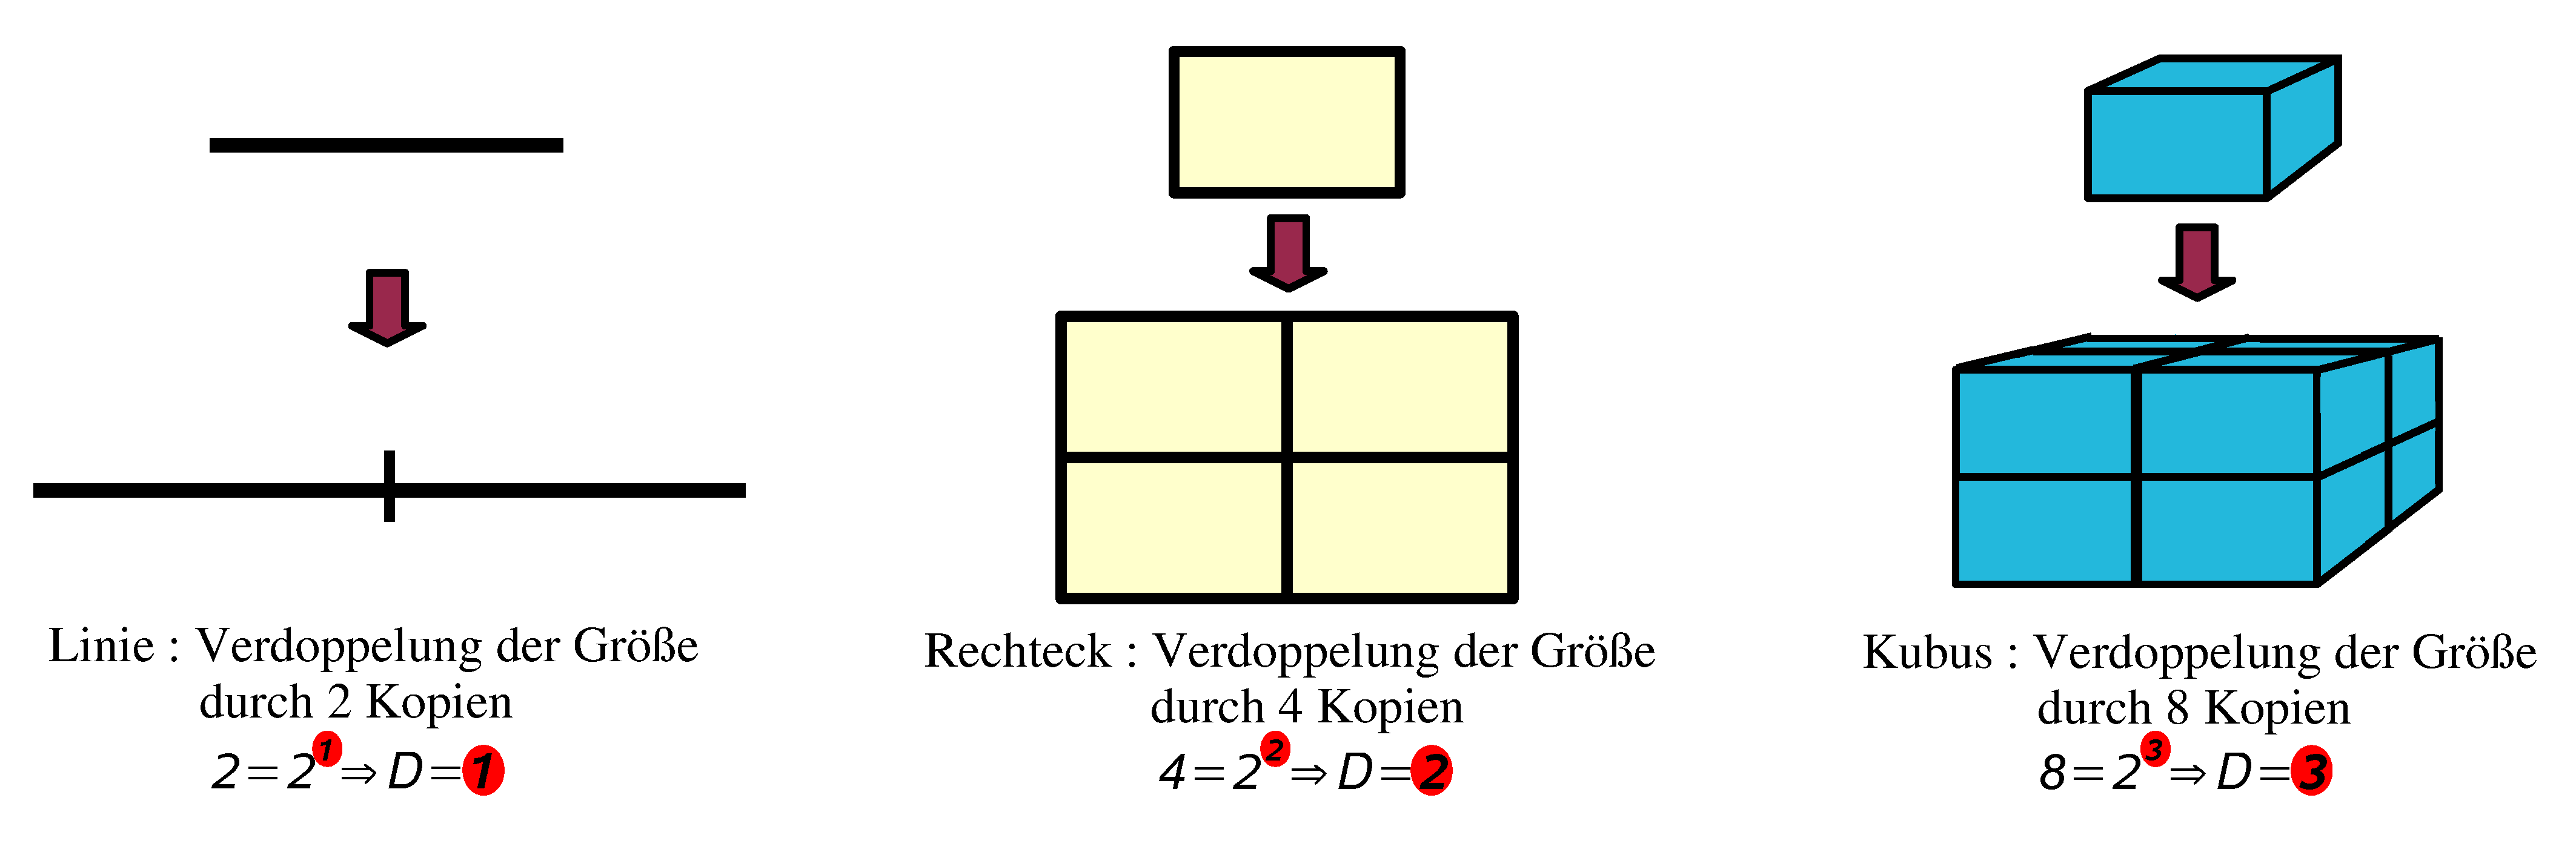
\includegraphics[width=1.01\textwidth]{fig/natD}\\[1.5cm]

    \begin{minipage}[c]{0.4\textwidth}\
      \textcolor{IPForange}{Allgemein} \\
      \textcolor{IPForange}{\textbf{Hausdorff Dimension}} 
    \end{minipage}\hfill
    \begin{minipage}[c]{0.01\textwidth}
      {\Huge :}
    \end{minipage}\hfill
    \begin{minipage}[c]{0.58\textwidth}
      \begin{center}
        F\"ur die $n$-fache Vergr\"o\ss erung des Objekts:\\
        $\boldsymbol{G\to n\,G}$ ben\"otigt man $\boldsymbol{N=n^D}$ Kopien
      \end{center}
    \end{minipage}


  \end{textblock}
  %%--------------------------------------------------------------------------%%

  

\end{myCol}
% ---------------------------------------------------------%
% end the column
% \hspace*{\colsep}%
\hfill
% ---------------------------------------------------------%
% second column
\begin{myCol}
  
%%--------------------------------------------------------------------------%%

  \begin{textblock}{Fraktale Dimensionen}
    \Large
  \begin{itemize} \setlength\itemsep{1.1em} \Large
    \item F\"ur kompliziertere oder allgemeinere Objekte \\
    \hspace*{4cm}fraktale \textbf{Haussdorf Dimension} $D_\text{f}$ sehr n\"utzlich
    \item Verallgemeinerung Dimensionsbegriff auf \textcolor{IPForange}{\textbf{nicht-ganzzahlige}} Werte
  \end{itemize}
  \vspace*{1.5cm}
  Aus \textcolor{IPForange}{$N=n^D$} folgt, dass \textcolor{IPForange}{$\ln N=D\,\ln n$}  und somit:
  \begin{align*}
    \color{IPForange}{\boldsymbol{ D \simeq \frac{\ln N(n)} {\ln n}}}
  \end{align*}

  \begin{minipage}[t]{0.38\textwidth}
    \begin{center}
      \textbf{Koch-Kurve}\\[1cm]
      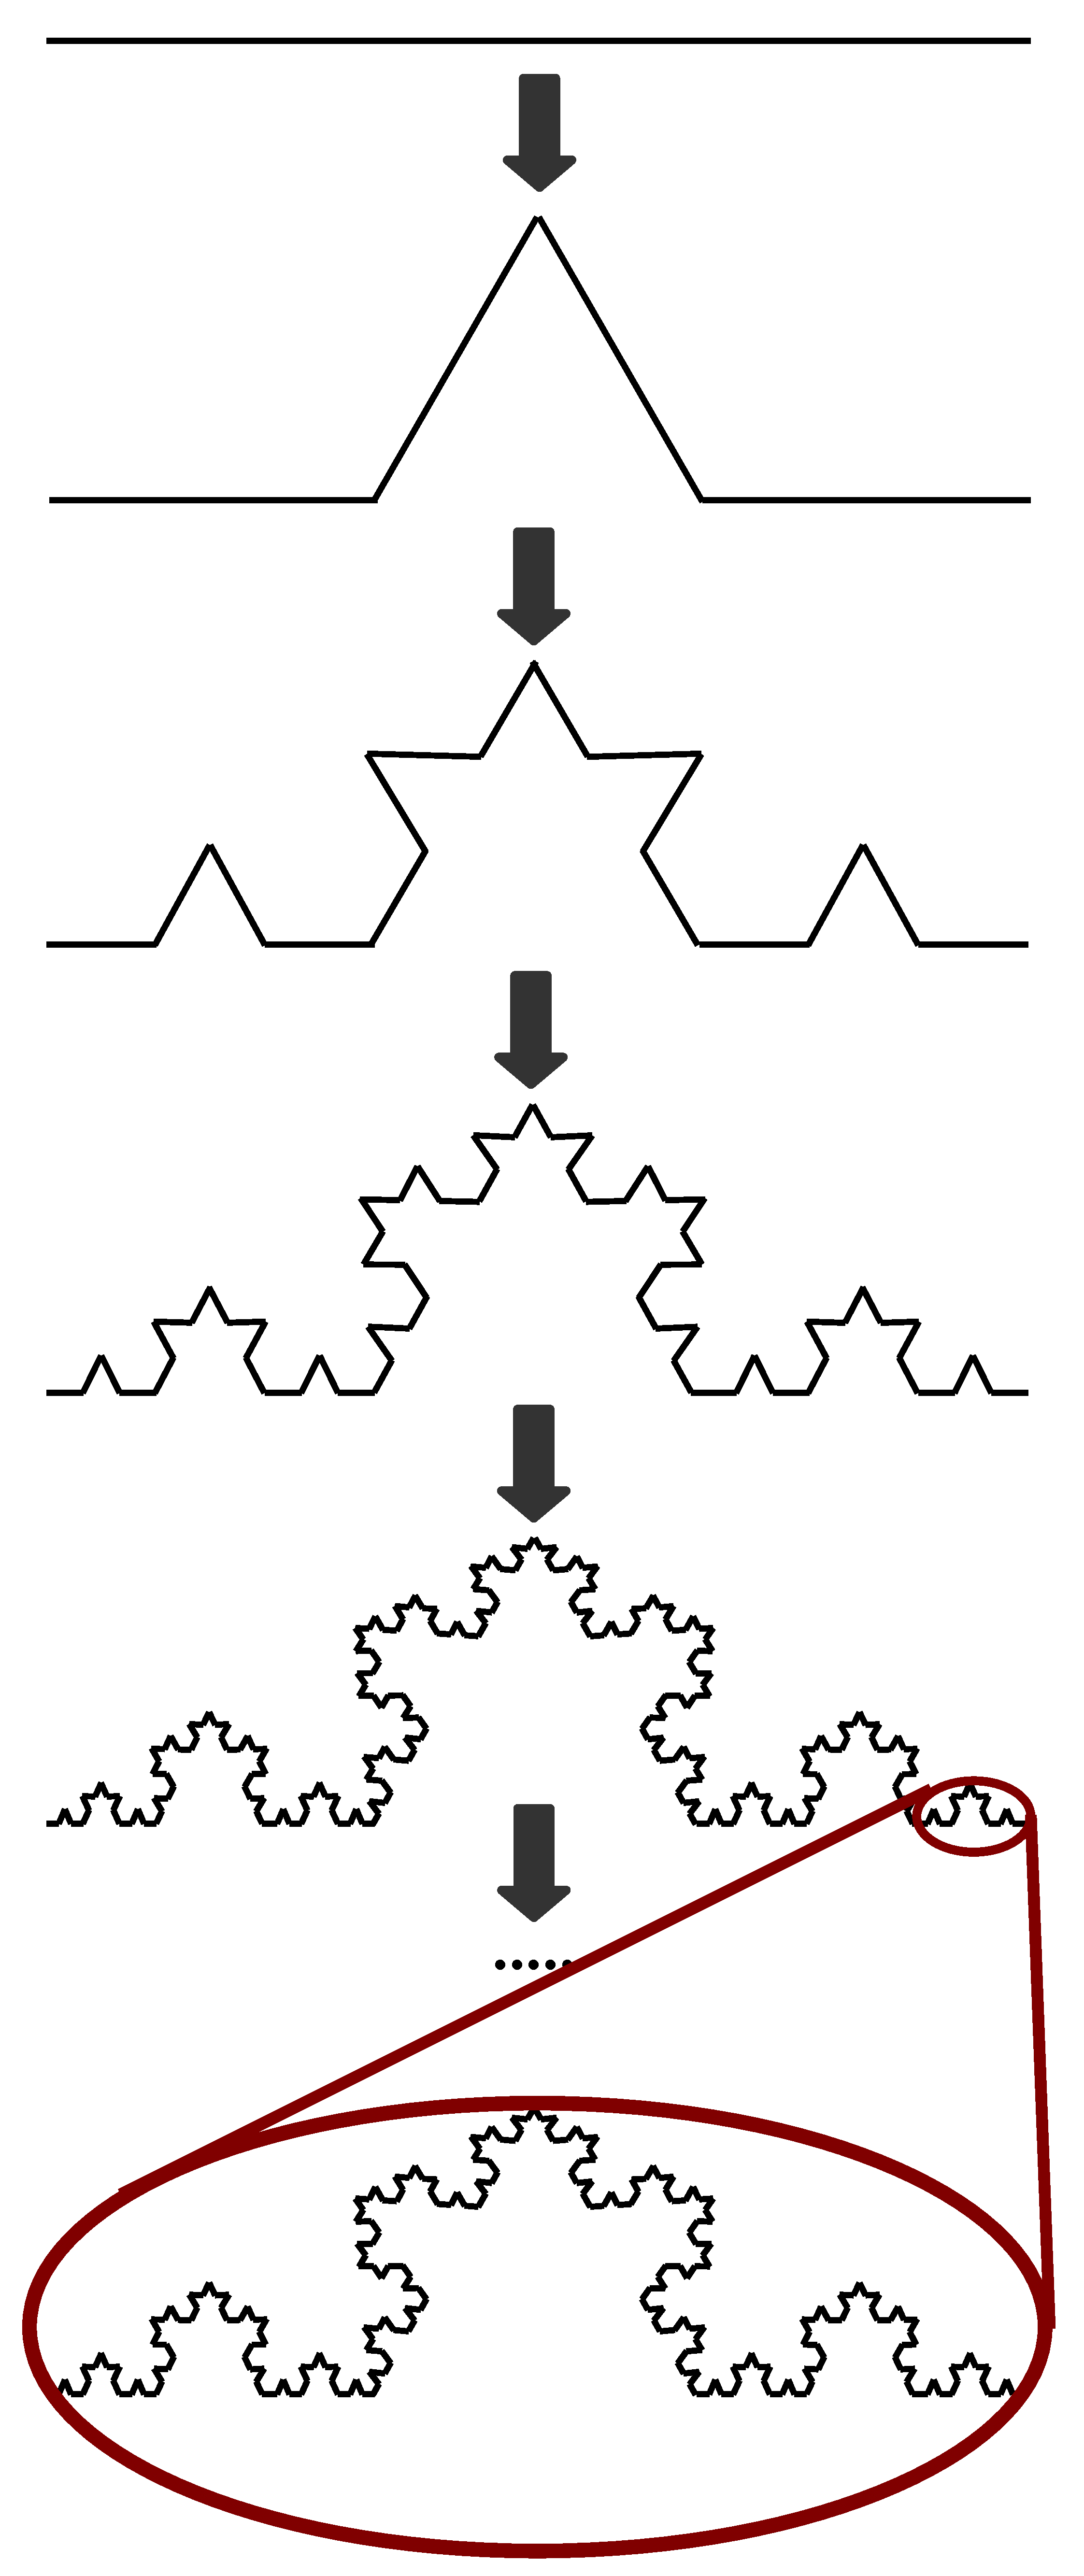
\includegraphics[width=0.9\textwidth]{fig/Koch3}
    \end{center}
  \end{minipage}\hfill
  \begin{minipage}[t]{0.58\textwidth}
    \vspace*{1.5cm}
    \textbf{ Konstruktion:}
    \begin{itemize} \setlength\itemsep{1.1em} \Large
      \item Schneide mittleres Drittel einer Linie aus
      \item Setze zwei Geraden als Zacke hinein
      \item Wiederholen an allen Geraden $\to\infty$
      \item \textcolor{IPForange}{$\rightarrow$} nach jedem Schritt ist Kurve um\\
      den Faktor $4/3$ l\"anger
      \item \textcolor{IPForange}{$\Rightarrow$} \textbf{unendlich lang}, aber auf \textbf{endliche Fläche beschränkt}
      \item \textit{Zoomen} zeigt immer gleiche Struktur\\[1.2em]
      \textcolor{IPForange}{\textbf{$\Rightarrow$}} Objekt ist \textcolor{IPForange}{\textbf{ selbst\"ahnlich}}
    \end{itemize}
    Gr\"o\ss e der Koch-Kurve wird ver-\textcolor{IPForange}{\textbf{drei}}-facht indem \textcolor{IPForange}{\textbf{vier}} Kopien konsturiert werden
    \begin{align*}
      {\color{IPForange}{\boldsymbol{\Rightarrow}}} {\color{IPFred}{ D }} =\frac{\ln 4}{\ln 3}\approx  \color{IPFred}{1,26}
    \end{align*}
  \end{minipage}

  \begin{minipage}[c]{0.58\textwidth}
    \vspace*{1.0cm}
    \textbf{ Konstruktion:}
    \begin{itemize} \setlength\itemsep{1.1em} \Large
      \item Schneide von geviertelten Dreieck das Zentrale heraus
      \item Wiederhole mit neuen Dreiecken $\to\infty$
      \item \textcolor{IPForange}{$\rightarrow$} jeder Schritt reduziert die Fläche\\
      um den Faktor $3/4$
      \item \textcolor{IPForange}{$\Rightarrow$} Fläche geht \textbf{gegen null}, aber Objekt hat \textbf{unendlichen Rand}
      \textcolor{IPForange}{\textbf{$\Rightarrow$}} Objekt ist ein \textcolor{IPForange}{\textbf{ selbst\"ahnlicher}}\textit{ Flickenteppich}\\[1.2em]
    \end{itemize}
      Gr\"o\ss e des Sierpinski-Dreiecks wird ver-\textcolor{IPForange}{\textbf{zwei}}-facht indem \textcolor{IPForange}{\textbf{drei}} Kopien konsturiert werden
      \begin{align*}
        {\color{IPForange}{\boldsymbol{\Rightarrow}}} {\color{IPFred}{ D }} =\frac{\ln 3}{\ln 2}\approx  \color{IPFred}{1,58}
      \end{align*}
    \end{minipage}
    \begin{minipage}[c]{0.35\textwidth}
      \begin{center}\vspace*{-5cm}
        \textbf{ Sierpinski-Dreieck}\\[1cm]
        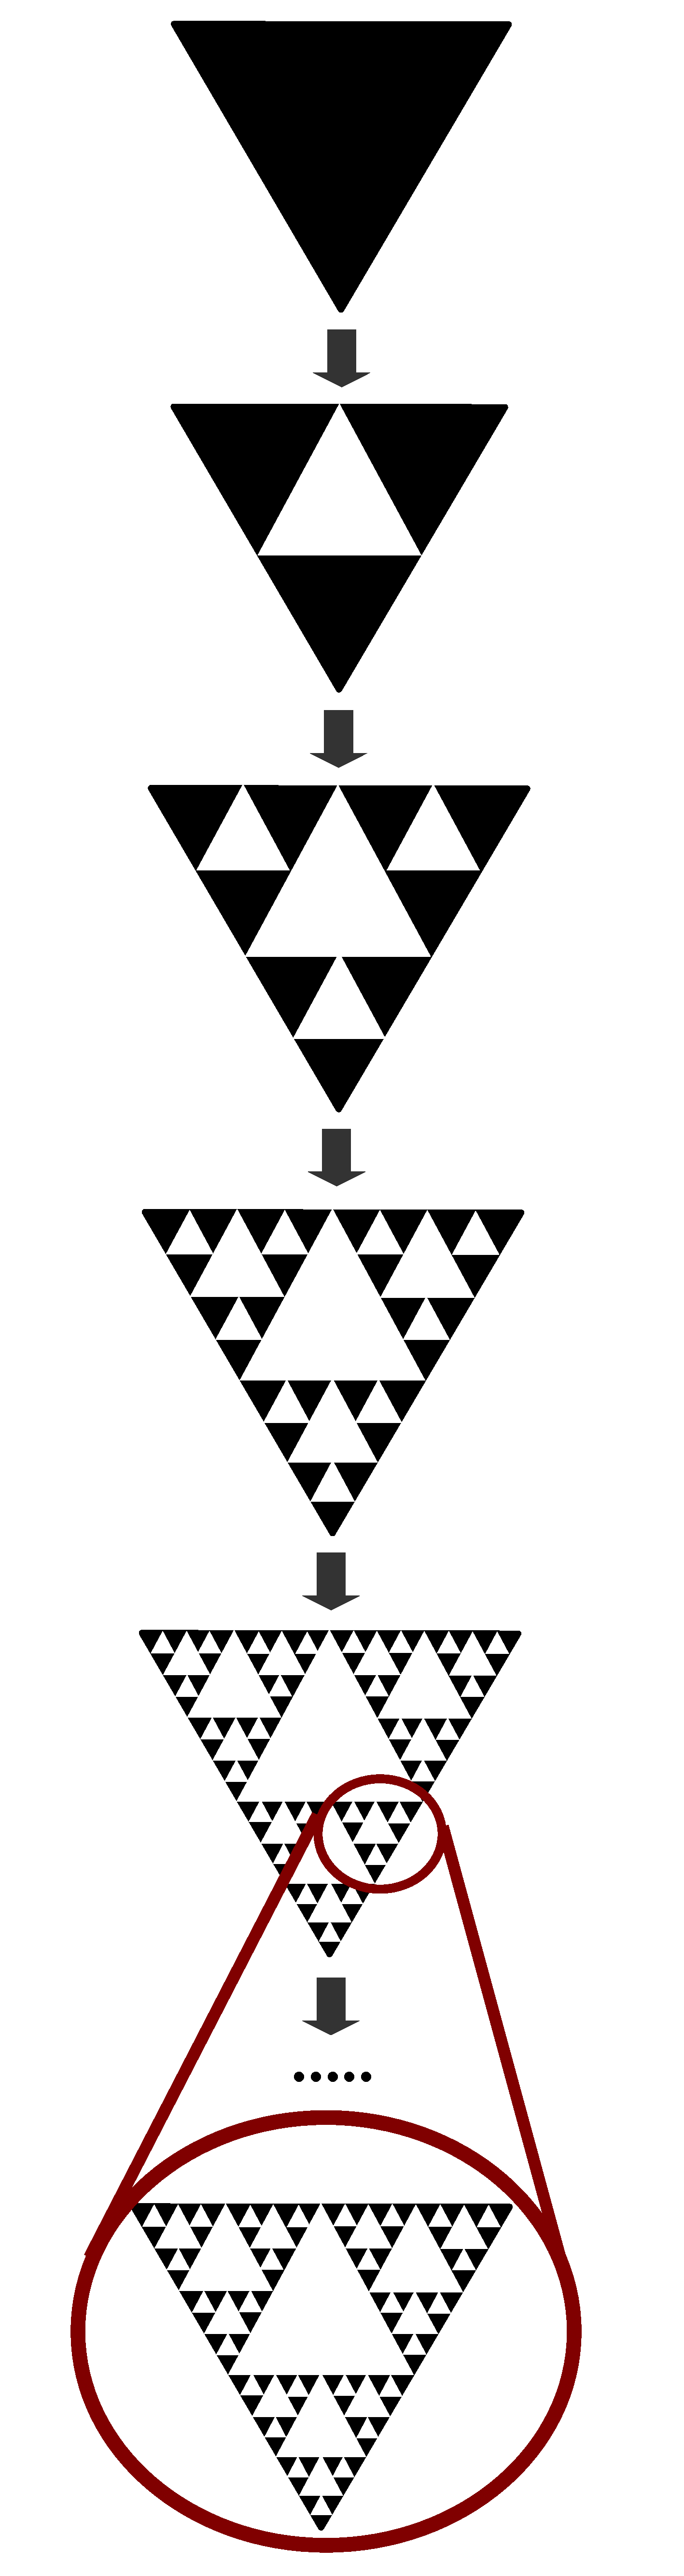
\includegraphics[width=0.5\textwidth]{fig/sierpinski2}
      \end{center}

  \end{minipage}
  %\end{center}

\end{textblock}
  %%--------------------------------------------------------------------------%%
  %%--------------------------------------------------------------------------%%


\end{myCol}%
\end{myTwoColPoster}
\end{frame}
\end{document}


%%% Local Variables:
%%% compile-command: "rake makepdf"
%%% End: